\documentclass[11pt]{article}

\usepackage[utf8]{inputenc}
\usepackage[T1]{fontenc}
\usepackage[francais]{babel}
\usepackage[top=1.8cm, bottom=1.8cm, left=1.8cm, right=1.8cm]{geometry}
\usepackage{hyperref}
\usepackage{graphicx}
\usepackage{epsfig}
\usepackage{array}
\hypersetup{
    colorlinks=true,
    breaklinks=true,
    urlcolor=red,
}
\parskip=5pt

\title{Organigramme}
\author{Pierre AYOUB, Claire BASKEVITCH, Tristan BESSAC, \\
Clément CAUMES, Damien DELAUNAY, Yassin DOUDOUH}
\date{Mercredi 14 Mars 2018}

\begin{document}
\hspace{1cm}
%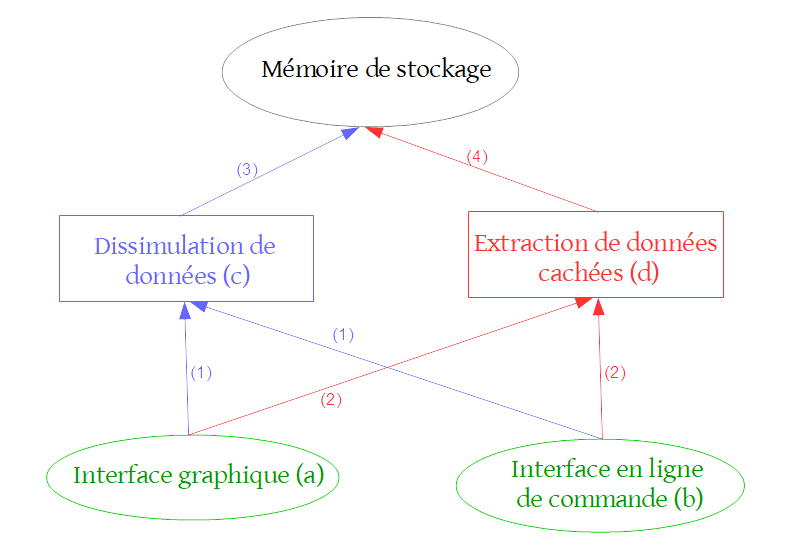
\includegraphics[scale=0.70]{organigramme.png}

\paragraph{Liste des modules et de leurs fonctionnalités}
\begin{description}
\item[a)] \textbf{Interface graphique / Interface en ligne de commande} : interfaces permettant à l'utilisateur de choisir parmi les deux fonctionnalités possibles de l'application. 
Il peut dissimuler des données dans un fichier (dont le type et le format sont pris en charge par l'application). Ou bien, il peut extraire les données cachées dans un fichier. 

\item[b)] \textbf{Compatibilité} : le format du fichier hôte (pour le module \textit{Dissimulation de données}) ou le format du fichier à analyser (pour le module \textit{Extraction de données cachées}), 
choisi par l'utilisateur, est vérifié pour savoir s'il est bien pris en charge par l'application. 

\item[c)] \textbf{Proposition des algorithmes de stéganographie} : en fonction du type et du format du fichier hôte, ainsi que de la taille des données à cacher, 
un ou plusieurs algorithmes seront proposés. 

\item[d)] \textbf{Détection de l'algorithme de stéganographie} : analyse du fichier pour découvrir quel algorithme a été utilisé afin de les extraire correctement par la suite. 

\item[e)] \textbf{Insertion des données} : la copie des données du fichier hôte sera modifiée avec l'insertion des données à cacher à l'aide de l'algorithme choisi par l'utilisateur. 

\item[f)] \textbf{Extraction} : les données cachées dans le fichier à analyser sont extraites. 

\end{description}

\paragraph{Liste des informations qui circulent entre les modules}
\begin{description}
\item[1)] 
\begin{itemize}
\item choix de l'utilisation de l'application (dissimulation ou extraction)
\item (nom du) fichier hôte, (nom du) fichier à cacher et chemin du fichier à créer (pour la dissimulation)
\item (nom du) fichier à analyser et chemin du fichier résultant de l'extraction des données cachées (pour l'extraction)
\end{itemize}
\item[2)] 
\begin{itemize}
\item (nom du) fichier hôte 
\item (nom du) fichier à cacher 
\item chemin du fichier à créer, qui dissimulera les données à cacher et ayant l'apparence de l'hôte. 
\end{itemize}
\item[3)] 
\begin{itemize}
\item (nom du) fichier contenant les données cachées à analyser
\item chemin du fichier résultant de l'extraction des données cachées
\end{itemize}
\item[4?)] 
\begin{itemize}
\item nom du fichier hôte 
\item nom du fichier à cacher
\end{itemize}
\item[5?)]
\begin{itemize}
\item fichier hôte
\item fichier à cacher 
\end{itemize}
\item[6?)]
\begin{itemize}
\item nom du fichier contenant les données cachées à analyser 
\end{itemize}
\item[7?)]
\begin{itemize}
\item fichier contenant les données cachées à analyser 
\end{itemize}
\item[8)]
\begin{itemize}
\item fichier hôte
\item fichier à cacher
\item chemin du fichier à créer lors de la dissimulation de données
\end{itemize}
\item[9)]
\begin{itemize}
\item fichier contenant les données cachées à analyser 
\item chemin du fichier résultant de l'extraction des données cachées
\end{itemize}
\item[10)]
\begin{itemize}
\item fichier hôte
\item fichier à cacher
\item chemin du fichier à créer lors de la dissimulation de données
\item nom de l'algorithme de stéganographie utilisé
\end{itemize}
\item[11)]
\begin{itemize}
\item fichier contenant les données cachées à analyser 
\item chemin du fichier résultant de l'extraction des données cachées
\item nom de l'algorithme détecté
\end{itemize}
\item[12)]
\begin{itemize}
\item données de l'hôte où les données à cacher ont été insérées en utilisant l'algorithme de stéganographie
\item chemin du fichier à créer lors de la dissimulation de données
\end{itemize}
\item[13)]
\begin{itemize}
\item données cachées extraites du fichier à analyser
\item chemin du fichier résultant de l'extraction des données cachées
\end{itemize}

\end{description}

\end{document}
